\documentclass[10.5pt,a4paper]{article}
\usepackage[margin=2.3cm]{geometry}
\usepackage[T1]{fontenc}
\usepackage{lmodern}
\usepackage{microtype}
\usepackage[htt]{hyphenat}
\emergencystretch=2em
\usepackage{amsmath,amssymb,bm}
\usepackage{graphicx}
\usepackage{booktabs}
\usepackage{siunitx}
\usepackage{xcolor}
\usepackage{enumitem}
\usepackage{caption}
\usepackage[section]{placeins}
\usepackage{tikz}
\usetikzlibrary{arrows.meta,positioning}
\usepackage[most]{tcolorbox}
\usepackage[colorlinks=true,linkcolor=blue!50!black,urlcolor=blue!50!black,citecolor=blue!50!black]{hyperref}
\sisetup{detect-all, per-mode=symbol, range-phrase=--}
\captionsetup{font=small,labelfont=bf}
\setlist{itemsep=2pt,topsep=4pt}
\definecolor{boxbg}{HTML}{F4F3F0}
\newtcolorbox{keybox}[1]{colback=boxbg,colframe=black!55,boxrule=0.5pt,arc=1pt,left=6pt,right=6pt,top=4pt,bottom=4pt,title=#1,fonttitle=\bfseries\small,coltitle=black,colbacktitle=boxbg}
\newcommand{\code}[1]{\texttt{#1}}
\newcommand{\zt}{\hat{\bm z}_t}
\newcommand{\gp}{g_{+}}
\newcommand{\gm}{g_{-}}

\title{\textbf{Tilted In-Hand Regrasping with Reinforcement Learning}\\[3pt]
\large Environment, control stack, reward design and learned policy\\
for the Franka regrasp task in Genesis, with the grasp axis tilted by $\theta\in[0^\circ,45^\circ]$}
\author{Genesis regrasp project}
\date{24 September 2026}

\begin{document}
\maketitle

\begin{keybox}{Summary}
\begin{itemize}[leftmargin=12pt]
\item \textbf{Task.} A \SI{35}{g}, $25\times25\times\SI{150}{mm}$ bar is held between the fingers. The policy has to
move it \SIrange{12.5}{22.5}{mm} along its own axis inside the hand. It does this by throwing: it moves the hand
along the grasp axis and fires short gripper pulses. \code{env\_franka\_parallel\_tilted.py} tilts that axis by a
fixed $\theta$ up to $45^\circ$ and keeps observations, reward and termination in a fixed task frame. At
$\theta=0$ it reproduces the original environment exactly. The unit tests confirm that observations match a
rotated copy of the original for $\theta\in\{0,15,30,45\}^\circ$.
\item \textbf{Policy.} A GRU actor-critic trained with PPO. The best tilted run (\code{tilt45-gru-speed},
$45^\circ$, domain randomization on) ends \SI{95.6}{\%} of training episodes in success over its last 50
iterations, with mean episode length \SI{3.7}{s}. Of the remaining episodes, \SI{3.6}{\%} fail, and
\SI{92}{\%} of those failures are the seventh-regrasp limit.
\item \textbf{Strategy.} The policy rises to the \SI{0.45}{m/s} velocity cap, fires the pulse so the gripper opens
as the command reverses at the \SI{15}{m/s^2} acceleration cap, and closes again while the hand moves down.
The bar keeps its upward momentum and moves up the hand. Each throw moves it \SIrange{10}{12}{mm} at
$45^\circ$ and costs several centimetres of hand height.
\item \textbf{Physics.} A 1-D model of the release reproduces Genesis' slip within \SI{0.3}{mm} at $0^\circ$, and
within \SI{0.2}{mm} at $40^\circ$--$45^\circ$ at the nominal friction ($\SI{3}{mm}$ across $\mu\in[0.25,1]$). It needs gravity along the axis \emph{and} friction on the lower finger,
because the transverse part of gravity loads the lower finger (Section~\ref{sec:physics}). The model shows that
\SI{0.45}{m/s} is too slow for the policy's \SIrange{120}{160}{ms} release window. At \SI{0.65}{m/s} Genesis gives
\SI{24}{mm} per throw, independent of window length.
\item \textbf{Reward.} With $\gamma=0.99$, the \SI{1.2}{s} pulse lockout multiplies the discounted success reward by
$0.55$ for every extra pulse. So slip per pulse is the quantity that decides both episode length and return.
\end{itemize}
\end{keybox}

\tableofcontents

%==========================================================================
\section{Task and problem statement}
%==========================================================================
The Franka Panda holds a \SI{35}{g} bar ($25\times25\times\SI{150}{mm}$, MJCF friction 0.75) in a pinch grasp.
Let $r_z$ be the bar centre's position relative to the midpoint of the two fingertips, measured along the grasp
axis. At reset $r_z\approx0$, and each episode draws a target
$r_z^*\sim\mathcal U[\SI{12.5}{mm},\SI{22.5}{mm}]$ (a random sign with \code{--mix}, negative with
\code{--negative}). The fingers never let go for good. The only way to change $r_z$ is a short release while
the hand accelerates, followed by a re-grasp: a \emph{dynamic regrasp}.

The policy acts at \SI{50}{Hz} ($T=\SI{20}{ms}$). Its outputs are a velocity command along the grasp axis and
a gripper action that can only \emph{trigger} a fixed-shape pulse. Physics runs at \SI{1}{kHz}. The tilted
variant rotates the whole grasp, and therefore the direction of motion, by an angle $\theta$ away from vertical.
The rotation is fixed for a run, and $\theta$ is not observed. Training in this report uses $\theta=45^\circ$,
the largest supported tilt.

%==========================================================================
\section{The tilted environment}
%==========================================================================
\subsection{Home posture: inverting joint 5}
The untilted home is $\bm q_0=(0,-0.82,0,-2.18,0,2.9,0.78)$~rad, with the grasp axis vertical. Tilting is done
with joint~5 alone. At home its axis $\hat{\bm a}$ is not horizontal ($a_z\neq0$), so $q_5=-\theta$ would give
the wrong inclination. Rotating the vertical $\hat{\bm e}_z$ by $q$ about $\hat{\bm a}$ (Rodrigues' formula)
gives
\begin{equation}
\hat{\bm e}_z\!\cdot\! R(\hat{\bm a},q)\,\hat{\bm e}_z=a_z^2+(1-a_z^2)\cos q=\cos\theta
\quad\Longrightarrow\quad
q_5(\theta)=-\arccos\frac{\cos\theta-a_z^2}{1-a_z^2}.
\end{equation}
$\hat{\bm a}$ is read from forward kinematics at start-up (\code{\_configure\_home\_pose}). With the unit-test
fixture $a_z=\cos1.36=0.21$, this gives $q_5=-15.3^\circ,-30.7^\circ,-46.1^\circ$ for
$\theta=15^\circ,30^\circ,45^\circ$. The test \code{test\_joint\_angle\_produces\_requested\_inclination} checks
the inversion to $10^{-7}$ degrees.

\subsection{Fixed task frame}
The frame is fixed at home and does not follow tracking errors. Let $q_{\text{f}}=q_{\text{EE}}(\theta)\otimes
q_{\text{EE}}(0)^{-1}$ be the change of hand orientation that the tilt produces. The task axes are the world axes
rotated by it, $A=[\hat{\bm x}_t\ \hat{\bm y}_t\ \zt]=R(q_{\text{f}})$, so $A=I$ exactly at $\theta=0$. With
$\bm p_0$ the hand position at home and $Z_0=\code{HOME\_TASK\_Z}=\SI{0.8546}{m}$,
\begin{equation}
z_t(\bm p)=Z_0+\zt^{\!\top}(\bm p-\bm p_0),\qquad \bm v_t=A^{\!\top}\bm v,\qquad
\bm r=A^{\!\top}\bigl(\bm p_{\text{bar}}-\tfrac12(\bm p_{\text{tip},l}+\bm p_{\text{tip},r})\bigr).
\label{eq:frame}
\end{equation}
Every observation, reward distance, success and failure bound, and hold target is expressed through
\eqref{eq:frame}. Gravity stays world-down, so in task coordinates it has an axial part $-g\cos\theta$ and a
transverse part of magnitude $g\sin\theta$. At $45^\circ$ Genesis gives
$A^{\!\top}\bm g=(-0.61,\,6.91,\,-6.94)\,\si{m/s^2}$. The transverse part lies along the finger-closing axis
(cosine $-0.996$), so the bar rests on the \emph{lower} finger whenever the grip opens (Figure~\ref{fig:geom}). The
consequences are worked out in Section~\ref{sec:physics}.

\begin{figure}[!htb]
\centering
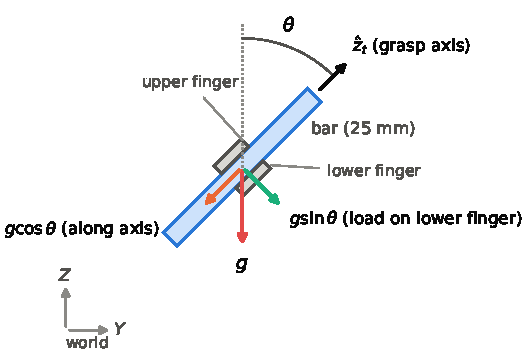
\includegraphics[width=0.58\linewidth]{figs/geometry.pdf}
\caption{Tilted grasp in the plane of the tilt. Gravity splits into $g\cos\theta$ along the grasp axis and
$g\sin\theta$ across it. In this posture the transverse part points along the finger axis, so an open grip leaves
the bar resting on the lower finger.}
\label{fig:geom}
\end{figure}

\subsection{Observation and action}
The observation layout is identical to the untilted environment, so existing policies load unchanged. With
\code{--normalization}, each channel is divided by the fixed scale below. With \code{--randomize},
$\mathcal U(\pm\SI{1}{mm})$ noise (or $\pm\SI{1}{mm/s}$) is added to channels 0, 1, 6, 7 and 8.
\begin{center}\small
\begin{tabular}{clll}
\toprule
idx & symbol & definition & scale\\
\midrule
0 & $z_t$ & hand position along the axis, Eq.~\eqref{eq:frame} & 1.0\\
1 & $\dot z_t$ & hand velocity along the axis, $\zt^{\!\top}\bm v_{\text{EE}}$ & 0.6\\
2, 3 & $v_k,\ a_k$ & current velocity reference and its step acceleration & 0.6, 15\\
4, 5 & $|\bm F_l|,|\bm F_r|$ & net contact-force magnitude on each finger & 5, 5\\
6, 7, 8 & $r_z, r_x, r_y$ & bar relative to the fingertip midpoint, task frame & 0.05\\
9 & $r_z^*$ & target in-hand offset & 0.05\\
\bottomrule
\end{tabular}
\end{center}
The action is $\bm a\in[-1,1]^3$. The first component sets the velocity reference and the other two set the
finger targets $p_f=p_{\min}+\tfrac12(a+1)(p_{\max}-p_{\min})$, with $p_{\min}=\SI{0.251}{mm}$ and
$p_{\max}=\SI{13.0}{mm}$ per finger. The open gap of \SI{26}{mm} clears the bar by \SI{0.5}{mm} per side.
Outside a pulse the fingers are clamped to $p_{\min}$, so the finger action serves only as a pulse trigger
(Section~\ref{sec:pulse}).

\subsection{From action to motion}
\paragraph{Reference.} The velocity command is scaled and then rate-limited:
\begin{equation}
v_k=\operatorname{clip}\!\bigl(a_{0}v_{\max},\,v_{k-1}\pm a_{\max}T\bigr),\qquad v_{\max}=\SI{0.45}{m/s},\ a_{\max}=\SI{15}{m/s^2}.
\end{equation}
The position knot is integrated with the trapezoid rule, and the step acceleration is the finite difference:
\begin{equation}
z_k=z_{k-1}+\tfrac12(v_{k-1}+v_k)T,\qquad a_k=(v_k-v_{k-1})/T.
\end{equation}
At \SI{1}{kHz} the reference is the cubic Hermite spline through $(z_{k-1},v_{k-1})$ and $(z_k,v_k)$,
$z(s)=h_{00}z_{k-1}+h_{10}Tv_{k-1}+h_{01}z_k+h_{11}Tv_k$ with $s\in[0,1]$.

\emph{Lemma.} With trapezoid-consistent knots, the Hermite velocity is exactly the linear interpolation of the
knot velocities, and its acceleration is exactly $a_k$:
\begin{equation}
\dot z(s)=(1-s)\,v_{k-1}+s\,v_k,\qquad \ddot z=a_k .
\end{equation}
\emph{Proof.} Differentiate:
$T\dot z=h_{00}'z_{k-1}+h_{10}'Tv_{k-1}+h_{01}'z_k+h_{11}'Tv_k$. Using $h_{01}'=-h_{00}'=6s-6s^2$ and substituting
$z_k-z_{k-1}=\tfrac12(v_{k-1}+v_k)T$, the $s^2$ terms cancel and the rest collects to
$T[(1-s)v_{k-1}+sv_k]$. $\square$

So the observed $a_k$ is the true reference acceleration. The reference jerk is impulsive at every knot, and that
is what the command filter smooths.

\paragraph{Command filter.} The velocity reference passes through
$H(s)=\omega_n^2/(s^2+2\zeta\omega_ns+\omega_n^2)$, with $\omega_n=\SI{75}{rad/s}$ and $\zeta=0.33$, tuned
against the real arm. It is discretized at $T_s=\SI{1}{ms}$ with the Tustin substitution
$s\mapsto\kappa\frac{1-z^{-1}}{1+z^{-1}}$, $\kappa=2/T_s$:
\begin{equation}
\alpha_0=\kappa^2+2\zeta\omega_n\kappa+\omega_n^2,\quad
b_0=b_2=\frac{\omega_n^2}{\alpha_0},\ b_1=\frac{2\omega_n^2}{\alpha_0},\quad
a_1=\frac{2\omega_n^2-2\kappa^2}{\alpha_0},\ a_2=\frac{\kappa^2-2\zeta\omega_n\kappa+\omega_n^2}{\alpha_0}.
\end{equation}
Its low-frequency delay is $2\zeta/\omega_n=\SI{8.8}{ms}$ and its step overshoot is
$e^{-\pi\zeta/\sqrt{1-\zeta^2}}=\SI{33}{\%}$. The overshoot matters for the throw: a commanded
$+0.45\to-0.45$ reversal becomes a hand swing of about $+0.47\to\SI{-0.61}{m/s}$ (Figure~\ref{fig:control}b).

\paragraph{Cartesian controller.} This runs at \SI{1}{kHz}. With $e=\bm p^{\text{ref}}-\bm p_{\text{EE}}$ and the
axial projector $P=\zt\zt^{\!\top}$, the commanded twist is
\begin{equation}
\bm v^{\text{cmd}}=\zt\,\tilde v+K_{\text{ax}}P\bm e+K_{\text{tr}}(I-P)\bm e,\qquad
\bm\omega^{\text{cmd}}=K_r\,\mathrm{rotvec}(q^{\text{ref}}\otimes q_{\text{EE}}^{-1}).
\end{equation}
Here $\tilde v$ is the filtered reference, $K_{\text{ax}}=8$, $K_{\text{tr}}=80$ and $K_r=\SI{40}{s^{-1}}$. It is
mapped to joint velocities with damped least squares,
$\dot{\bm q}=J^{\!\top}(JJ^{\!\top}+\lambda I)^{-1}[\bm v^{\text{cmd}};\bm\omega^{\text{cmd}}]$ with
$\lambda=10^{-4}$, and tracked by the joint velocity loop ($k_v=0.35\times$ nominal, torque limits
\SI{87}{Nm}/\SI{12}{Nm}). The transverse gain is ten times the axial gain so the hand stays on the tilted line
against the gravity-induced sideways drift. The axial loop is unchanged from the untilted environment. The
unit test \code{test\_control\_holds\_orientation\_and\_commands\_axis\_velocity} checks that a lateral offset
and a yaw error produce restoring commands without changing the axial speed.

\begin{figure}[!htb]
\centering
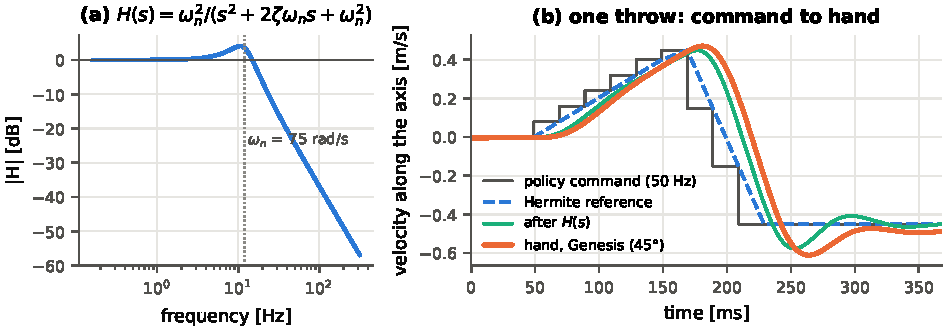
\includegraphics[width=\linewidth]{figs/control_chain.pdf}
\caption{(a) Magnitude of the command filter. (b) One throw at $45^\circ$: the \SI{50}{Hz} policy command, the
Hermite reference (a linear ramp inside each step, by the Lemma), the filtered reference, and the hand velocity
Genesis measures. The hand overshoots the \SI{-0.45}{m/s} command to \SI{-0.61}{m/s}.}
\label{fig:control}
\end{figure}

\subsection{Gripper pulse}\label{sec:pulse}
A pulse fires on a rising edge of the \emph{effective} mean finger command through the mid-position. Pulses are
blocked during the first 50 steps (\SI{1}{s}) and for $N_\ell=60$ steps (\SI{1.2}{s}) after the previous trigger.
On a trigger the counter is set to $c=L+D$, with $D=2$ and $L=7$. For $c>L$ the policy's command passes through
(this is the delay). For $2\le c\le L$ the fingers are forced open for $L-1=6$ steps (\SI{120}{ms}). At $c=1$ they
are forced closed. Afterwards they are clamped closed. If the policy keeps commanding ``open'' through the
delay, the bar can be loose for up to $(D+L-1)T=\SI{160}{ms}$. Because the edge detector remembers the
effective command, holding ``open'' through the lockout still produces an edge the moment the lockout ends.
Figure~\ref{fig:timing} shows the pulse together with the reward windows keyed to the trigger.

\begin{figure}[!htb]
\centering
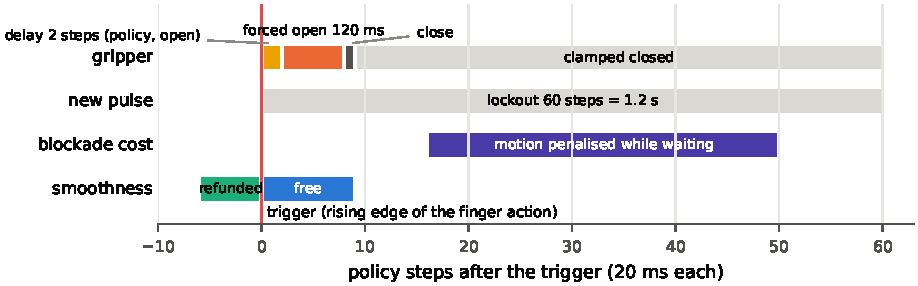
\includegraphics[width=\linewidth]{figs/pulse_timing.pdf}
\caption{Pulse state machine and the reward windows attached to the trigger (current constants). The smoothness
refund and exemption are defined in Section~\ref{sec:smooth}, the blockade window in Section~\ref{sec:speed}.}
\label{fig:timing}
\end{figure}

\subsection{Termination and randomization}
\textbf{Success} requires all of the following for 5 consecutive steps: $|r_z-r_z^*|\le\SI{5}{mm}$,
$|\dot z_t|<\SI{0.05}{m/s}$, a firm grasp (mean finger force $\bar F\ge\SI{0.75}{N}$) for at least 3 steps, and
$z_t\in[0.70,0.86]$~m. \textbf{Failure} is any of $|r_x|$ or $|r_y|>\SI{40}{mm}$, fingertip distance
$<\SI{10}{mm}$, $|r_z|>\SI{150}{mm}$, $z_t\notin[0.60,0.96]$~m, or a seventh regrasp. \textbf{Timeout} is 450 steps
(\SI{9}{s}). Every reset samples the finger gain $k_p\sim\mathcal U[100,500]$ (force limit $=k_p$) and the contact
friction $\mu\sim\mathcal U[0.6,0.9]$, whether or not \code{--randomize} is set. \code{--randomize} adds the
observation noise above and initial joint-velocity noise of $\pm\SI{0.01}{rad/s}$. The pulse delay is fixed at two
steps in every mode.

%==========================================================================
\section{Reward}
%==========================================================================
The per-step reward is a weighted sum. Only the keys of \code{REWARD\_TERM\_WEIGHTS} are summed:
\begin{equation}
r=r_{\text{base}}+r_{\text{prox}}+2\,r_{\text{regrasp}}+r_{\text{acc}}+r_{\text{jerk}}+r_{\text{flip}}+r_{\text{blockade}}+r_{\text{speed}},
\end{equation}
with $r_{\text{flip}}\equiv0$ at present, because its coefficient is 0. The post-pulse hold penalty is computed
for its countdowns but is not summed. Figure~\ref{fig:rewards} plots each term.

\subsection{Terminal and base reward}
\begin{equation}
r_{\text{base}}=\begin{cases}
R_s-c_tk & \text{success at step }k,\quad R_s=10^4,\ c_t=0.5\\
-F & \text{failure}\\
-R_{\text{to}} & \text{timeout},\quad R_{\text{to}}=250\\
-c_a & \text{otherwise},\quad c_a=1.25 .
\end{cases}
\end{equation}
Undiscounted, failing at step $t$ returns $-c_a(t-1)-F$ and timing out returns $-c_a(L_{\max}-1)-R_{\text{to}}$.
Failing is strictly worse for every $t\ge1$ if and only if $F>R_{\text{to}}+c_a(L_{\max}-1)$. The code uses
$F=R_{\text{to}}+c_aL_{\max}+100=912.5$, derived in \code{fail\_penalty()}, so the ordering survives any change
to the constants.

\subsection{Proximity}
\begin{equation}
r_{\text{prox}}(d)=M\,\frac{e^{-kd/R}-e^{-k}}{1-e^{-k}},\qquad d=|r_z-r_z^*|,\ M=30,\ R=\SI{50}{mm},\ k=5,
\end{equation}
clipped to $[0,M]$. It pays 30, 18.1, 10.9 and 3.9 at $d=0$, 5, 10 and \SI{20}{mm}.\footnote{The comment above
\code{PROXIMITY\_REWARD\_MAX} still quotes the values for $M=20$.} It is dense but bounded, and
Section~\ref{sec:returns} shows that loitering cannot beat finishing.

\subsection{Regrasp bonus}
A \emph{release} starts when $\bar F<\SI{0.15}{N}$. A \emph{regrasp event} is the first step after a release
with $\bar F\ge\SI{0.75}{N}$. With $e_{\text{b}}$ and $e_{\text{a}}$ the target errors $|r_z-r_z^*|$ at the
release and at the regrasp, let $\delta=e_{\text{b}}-e_{\text{a}}$. Then
\begin{equation}
\rho(\delta)=7500\,\max(\delta,-0.05)\Bigl(\frac{|\delta|}{\SI{7.5}{mm}}\Bigr)^{3}\ \ \text{clipped above at }10^4,
\qquad r_{\text{regrasp}}=\begin{cases}\rho & \rho\ge0\\ 5\rho&\rho<0,\end{cases}
\end{equation}
paid only on the first four regrasps. The bonus is \emph{quartic}, $\propto\delta|\delta|^3$. Weighted by 2, it
pays 112.5, 356, 1800 and 5689 for improvements of 7.5, 10, 15 and \SI{20}{mm}. One \SI{20}{mm} regrasp therefore
earns eight times as much as two \SI{10}{mm} regrasps. Since $\delta\le e_{\text{b}}\le\SI{22.5}{mm}$ in a normal
episode, the weighted bonus stays below $9.1\times10^3$ and the cap (reached at $\delta=\SI{27.4}{mm}$) is not
binding. A worsening costs five times the bonus of the same improvement, so a deliberate
``worsen then improve'' cycle loses reward.

\subsection{Smoothness with pulse refunds}\label{sec:smooth}
\begin{equation}
r_{\text{acc}}=-25\Bigl(\frac{a_k}{a_{\max}}\Bigr)^2,\qquad r_{\text{jerk}}=-25\Bigl(\frac{a_k-a_{k-1}}{2a_{\max}}\Bigr)^2 .
\end{equation}
Both are at most 25 per step: a full-scale alternating acceleration costs 50 per step, or 1500 over 30 steps.
The throw needs exactly such accelerations, so both terms have a refund mechanism. On an \emph{accepted} trigger:
\begin{itemize}
\item the charges of the previous six steps are paid back once;
\item the trigger step and the next eight steps are free.
\end{itemize}
The run-up and the reversal are therefore free exactly when they lead to a real pulse, and cost full price
otherwise. The refund cancels the charges exactly in undiscounted terms. Under discounting a charge $j$ steps
before the refund keeps a residue $1-\gamma^j\le1-0.99^6=5.9\,\%$. Five unit tests pin the bookkeeping: the
window boundaries, no double refund, per-environment resets, and that a trigger rejected by the lockout refunds
nothing.

\subsection{Speed and blockade}\label{sec:speed}
With the measured speed above a \SI{0.02}{m/s} deadzone, $u=\max(|\dot z_t|-0.02,0)$,
\begin{equation}
r_{\text{speed}}=-2.25\Bigl(\frac{u}{v_{\max}}\Bigr)^2,\qquad
r_{\text{blockade}}=-\mathbb 1_{\text{idle}}\Bigl[\Bigl(\frac{u}{0.1}\Bigr)^2+0.25\Bigl(\frac{v_k}{0.1}\Bigr)^2\Bigr].
\end{equation}
$\mathbb 1_{\text{idle}}$ is 1 while no pulse is running, at least \SI{0.3}{s} have passed since the trigger
(settle), and more than \SI{0.2}{s} of the block remains (prep). That is steps 16--50 of each lockout, and steps
1--40 of an episode (Figure~\ref{fig:timing}). Motion is never free, but it is most expensive while the policy
waits for the next pulse.

\begin{figure}[!htb]
\centering
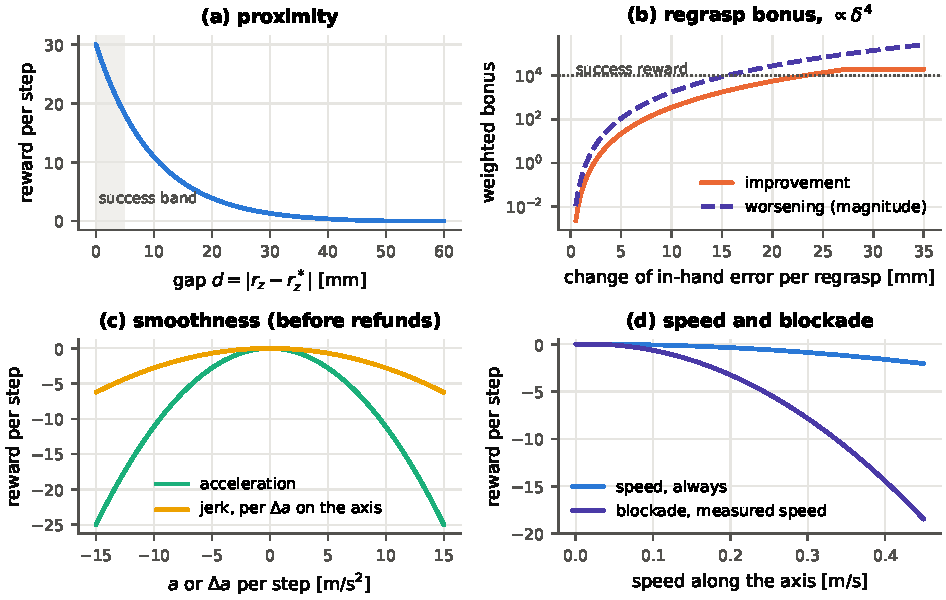
\includegraphics[width=\linewidth]{figs/reward_terms.pdf}
\caption{Reward terms with the current constants: (a) proximity; (b) weighted regrasp bonus on a log scale, where
improvement and worsening are $\propto\delta^4$ and worsening is five times heavier; (c) smoothness before
refunds; (d) speed and blockade penalties.}
\label{fig:rewards}
\end{figure}

\subsection{What the discount does to the design}\label{sec:returns}
PPO optimizes $\sum_k\gamma^kr_k$ with $\gamma=0.99$, an effective horizon of $1/(1-\gamma)=100$ steps
(\SI{2}{s}). The earliest success after $n$ pulses comes at step
$t_n\approx50+60(n-1)+12$: the start block, then one lockout per extra pulse, then settling. The discounted
terminal value falls by $\gamma^{60}=0.547$ per pulse. Figure~\ref{fig:returns} evaluates the base stream exactly.
Finishing after 1, 2, 3, 4 or 5 pulses is worth 5343, 2858, 1502, 763 and 359. Loitering to timeout at
\SI{6}{mm} from the target is worth 1493 (just outside the success band), and at \SI{12}{mm} it is worth 753.
\begin{itemize}
\item \textbf{A policy that needs four or more pulses gains nothing over hovering near the target}, before the
regrasp bonus is counted. The bonus, quartic in slip per pulse, points the same way.
\item \textbf{Slip per pulse is therefore the quantity that sets the return.} Section~\ref{sec:physics} shows
that it is limited by the \SI{0.45}{m/s} velocity cap, not by the policy.
\end{itemize}

\begin{figure}[!htb]
\centering
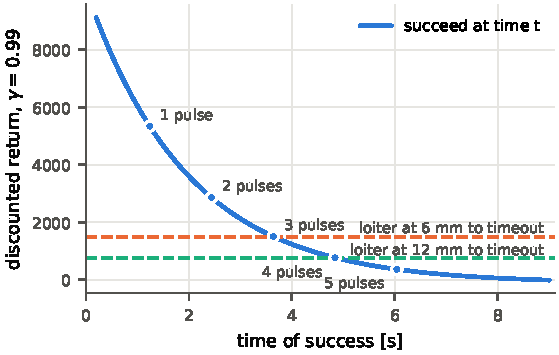
\includegraphics[width=0.62\linewidth]{figs/returns.pdf}
\caption{Discounted base return against the time of success (alive cost included), with the earliest success
after $n$ pulses marked. The dashed lines are loitering at a fixed distance until timeout.}
\label{fig:returns}
\end{figure}

%==========================================================================
\section{Learning}
%==========================================================================
\subsection{PPO with a recurrent actor-critic}
Training uses rsl\_rl~5 PPO. With $\rho_t=\pi_\theta(a_t|h_t)/\pi_{\text{old}}(a_t|h_t)$ and GAE advantages
\begin{equation}
\hat A_t=\sum_{l\ge0}(\gamma\lambda)^l\delta_{t+l},\qquad \delta_t=r_t+\gamma V(h_{t+1})-V(h_t),
\end{equation}
the minimized loss is
\begin{equation}
\mathcal L=\mathbb E\bigl[\max(-\rho_t\hat A_t,\,-\operatorname{clip}(\rho_t,1\pm\epsilon)\hat A_t)\bigr]
+c_V\,\mathbb E\bigl[\max\bigl((V-R)^2,(V_{\text{old}}+\operatorname{clip}(V-V_{\text{old}},\pm\epsilon)-R)^2\bigr)\bigr]
-c_H\,\mathbb E[\mathcal H(\pi_\theta)].
\end{equation}
The learning rate adapts to the measured KL divergence. It is divided by 1.5 (floor $10^{-5}$) when
$\mathrm{KL}>2\,\mathrm{KL}^*$ and multiplied by 1.5 (cap $10^{-2}$) when $\mathrm{KL}<\mathrm{KL}^*/2$.

\begin{center}\small
\begin{tabular}{llll}
\toprule
$\gamma,\ \lambda$ & 0.99, 0.95 & clip $\epsilon$ & 0.2\\
KL$^*$, initial lr & 0.01, $3\times10^{-4}$ & $c_V,\ c_H$ & 1.0, 0.005\\
epochs $\times$ minibatches & $5\times4$ & max grad norm & 1.0\\
actor & GRU(256) $\to$ MLP 256-128-64, ELU & action std & scalar, init 1.0\\
critic & GRU(256) $\to$ MLP 256-128-64 & rollout = BPTT horizon & 64 steps (\SI{1.28}{s})\\
\bottomrule
\end{tabular}
\end{center}

\paragraph{Why recurrent.} The observation contains no pulse phase, no lockout counter, no friction and no finger
gain, although all of them change what a good action is. The GRU state $h_t=\mathrm{GRU}(o_t,h_{t-1})$ can recover
them from history. For example, the slip the last pulse produced carries information about $\mu$. The
\SI{1.28}{s} BPTT window is just longer than one pulse cycle (60 steps), so the gradient can connect a trigger
to the regrasp it caused. Recurrent minibatches split environments rather than time, so each minibatch holds
whole 64-step sequences.

\subsection{Runs}
All runs below use $\theta=45^\circ$, \code{--normalization}, \code{--randomize} and positive targets.
\begin{center}\small
\begin{tabular}{lcccc}
\toprule
run & iterations & success, last 50 it. & best success (20-it. mean) & episode length\\
\midrule
\code{tilt45-gru} & 825 & \SI{64.6}{\%} & \SI{87.6}{\%} & \SI{5.6}{s}\\
\code{tilt45-gru-jerk} & 1014 & \SI{77.4}{\%} & \SI{86.7}{\%} & \SI{4.2}{s}\\
\code{tilt45-gru-speed} & 709 & \SI{95.6}{\%} & \SI{96.4}{\%} & \SI{3.7}{s}\\
\code{tilt45-gru-speed-only-up} & 418 & \SI{82.5}{\%} & \SI{85.8}{\%} & \SI{2.1}{s}\\
\bottomrule
\end{tabular}
\end{center}
These are training-time rates from the reward table, which uses the stochastic policy with randomization on.
The run directories store no source snapshot, so the runs record successive revisions of the reward (named at
training time) rather than a controlled ablation. The steps in Figure~\ref{fig:learning} coincide with resumes:
iteration 700 for \code{tilt45-gru}, 600 for \code{-jerk} and 620 for \code{-speed}. Where a resume lowered
the success rate, the curve settles at the new level rather than recovering. \code{tilt45-gru-speed} is the only
run above \SI{90}{\%}. Its residual failures are almost entirely the seventh-regrasp limit
(Figure~\ref{fig:failures}): the policy runs out of attempts, not out of stability. \code{-speed-only-up} has the
shortest episodes (\SI{2.1}{s}), consistent with the discount argument of Section~\ref{sec:returns}.

\begin{figure}[!htb]
\centering
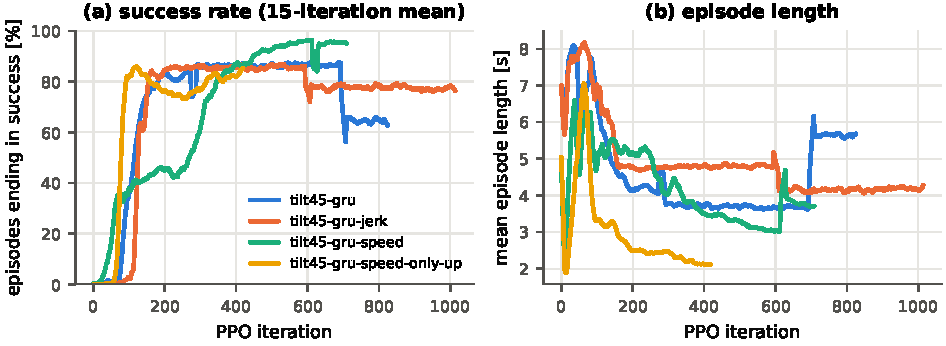
\includegraphics[width=\linewidth]{figs/learning.pdf}
\caption{Training curves of the four $45^\circ$ GRU runs (15-iteration moving mean).}
\label{fig:learning}
\end{figure}

\begin{figure}[!htb]
\centering
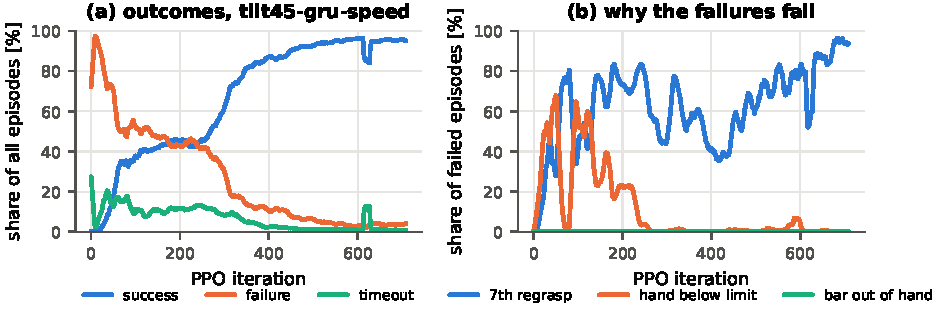
\includegraphics[width=\linewidth]{figs/failures.pdf}
\caption{\code{tilt45-gru-speed}. (a) Outcomes as a share of all episodes. (b) Failure reasons as a share of
failed episodes. The early failures are dominated by the hand leaving its height band; the late ones by the
seventh-regrasp limit.}
\label{fig:failures}
\end{figure}

%==========================================================================
\section{The learned strategy and its physics}\label{sec:physics}
%==========================================================================
\subsection{The throw}
Figure~\ref{fig:episode} shows the first \SI{1.36}{s} of the $45^\circ$ episode exported for the real cell
(\code{franka\_controllers/traj\_vis/tilt45/traj\_d2\_l5.csv}, \code{tilt45-gru}, checkpoint 820). The policy
drifts down slowly during the start block. It then rises to the \SI{0.45}{m/s} cap and fires so that the open
window starts at the step where the command reverses at the $\SI{-15}{m/s^2}$ cap. It re-grips at
\SI{-0.45}{m/s}. The bar gains \SI{11.2}{mm} in one throw, and the hand ends about \SI{50}{mm} lower along the
axis. After the throw the command alternates at $\pm\SI{15}{m/s^2}$ every step. This checkpoint predates the
smoothness revision, and that chatter is what the acceleration and jerk costs of later runs target.
Figure~\ref{fig:ep4} is an episode of \code{tilt45-gru-speed-only-up} with four throws. The bar climbs
$0\to6\to15\to18\to\SI{19}{mm}$ while the hand's lowest point falls from \SI{0.67}{m} to \SI{0.60}{m}. The
episode fails on the lower height limit. \textbf{Every throw spends hand height, so the height band caps the
number of throws at about four}, independently of the regrasp limit.

\begin{figure}[!htb]
\centering
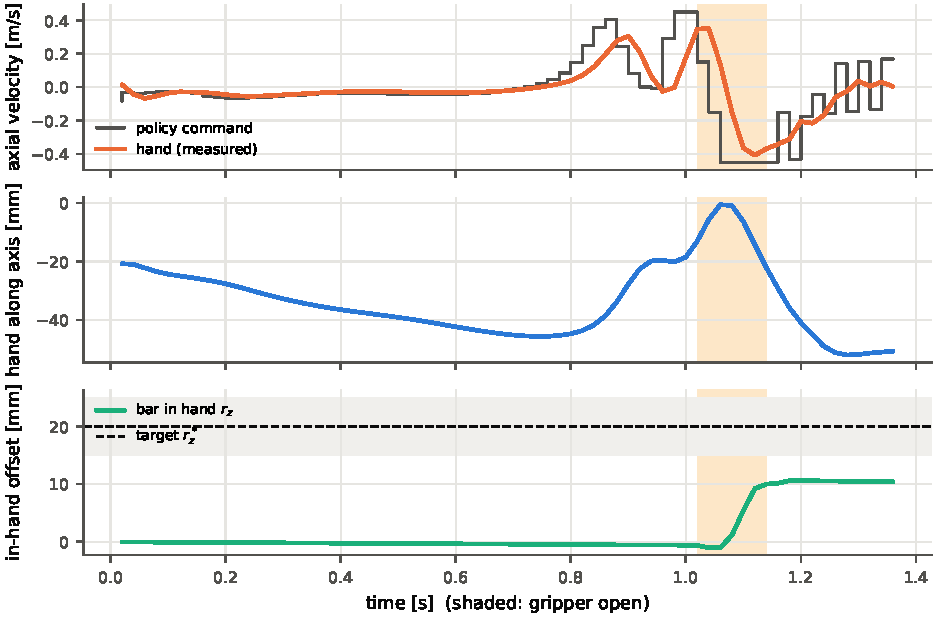
\includegraphics[width=\linewidth]{figs/episode.pdf}
\caption{First \SI{1.36}{s} of the exported $45^\circ$ trajectory; shading marks the open gripper. Top: policy
command and measured hand velocity along the axis. Middle: hand position along the axis. Bottom: in-hand offset,
with the target and its $\pm\SI{5}{mm}$ success band.}
\label{fig:episode}
\end{figure}

\begin{figure}[!htb]
\centering
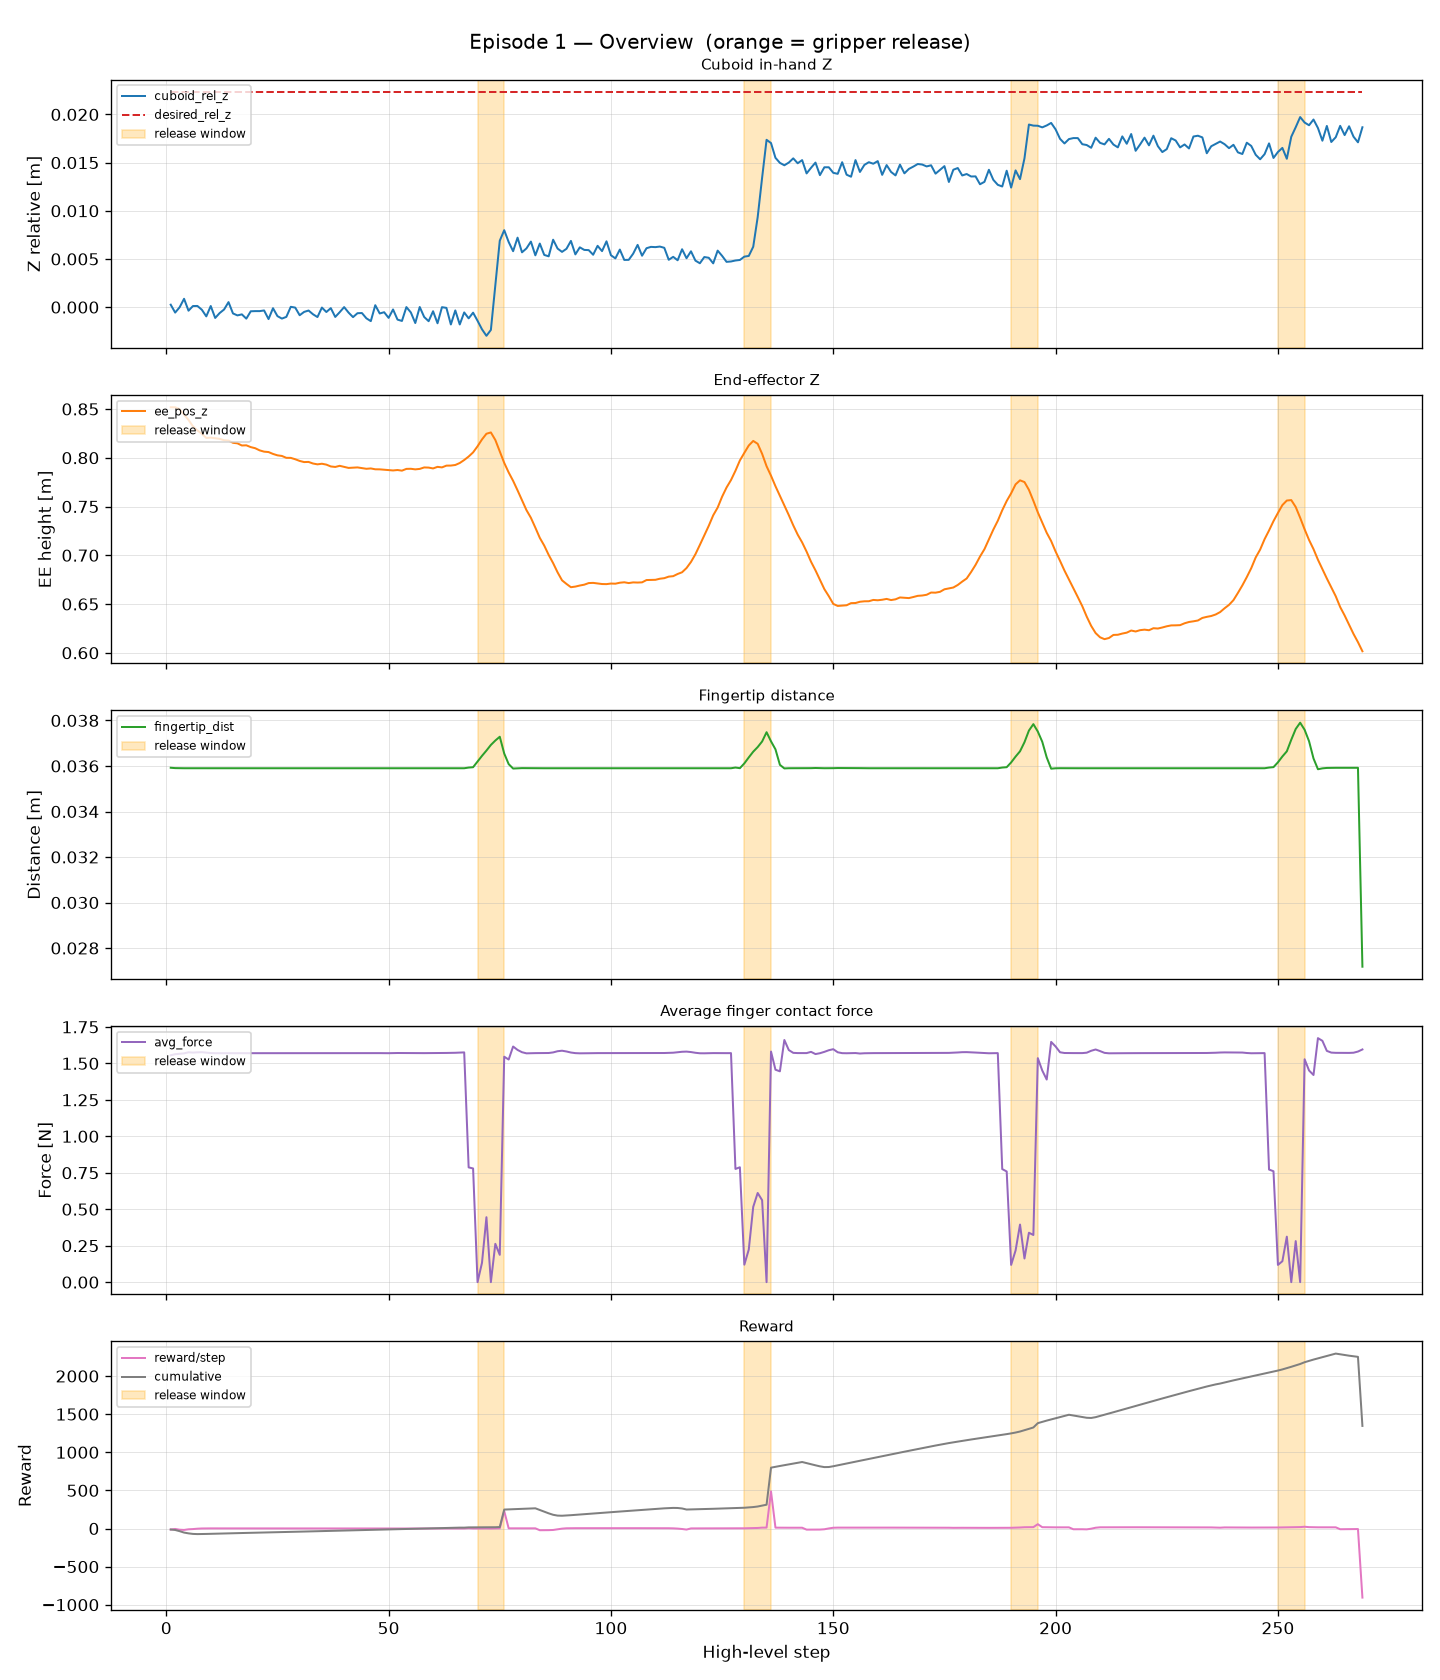
\includegraphics[width=0.9\linewidth]{figs/ep001_overview_speed_only_up.png}
\caption{An episode of \code{tilt45-gru-speed-only-up}, plotted by the project's evaluation tooling. Four throws
move the bar up in steps of \SIrange{3}{9}{mm} while the hand's lowest point sinks with each throw, until
$z_t<\SI{0.60}{m}$ ends the episode as a failure.}
\label{fig:ep4}
\end{figure}

\subsection{Why the bar moves: relative dynamics}
In the hand frame, with $w=v_{\text{bar}}-v_{\text{hand}}$ and slip $\Delta=\int w\,\mathrm dt$ after a release,
the bar rests on the lower finger (Figure~\ref{fig:geom}). Its motion relative to the hand is
\begin{equation}
\dot w=\begin{cases}-g(\cos\theta+\mu\sin\theta)-a_h & w>0\\ -g(\cos\theta-\mu\sin\theta)-a_h & w<0\\ 0 & w=0,\ |g\cos\theta+a_h|\le\mu g\sin\theta.\end{cases}
\label{eq:rel}
\end{equation}
The bar climbs the hand only while the hand decelerates faster than $\gp=g(\cos\theta+\mu\sin\theta)$, which is
\SI{12.1}{m/s^2} at $45^\circ$ with $\mu=0.75$. That explains why the policy uses its full \SI{15}{m/s^2} and
why the filter overshoot helps it. Integrated with Genesis' measured hand velocity, Eq.~\eqref{eq:rel}
reproduces the \SI{1}{kHz} slip trace (Figure~\ref{fig:physics}). Gravity along the axis alone would predict
\SI{29}{mm} instead of the \SI{12}{mm} observed.

\begin{figure}[!htb]
\centering
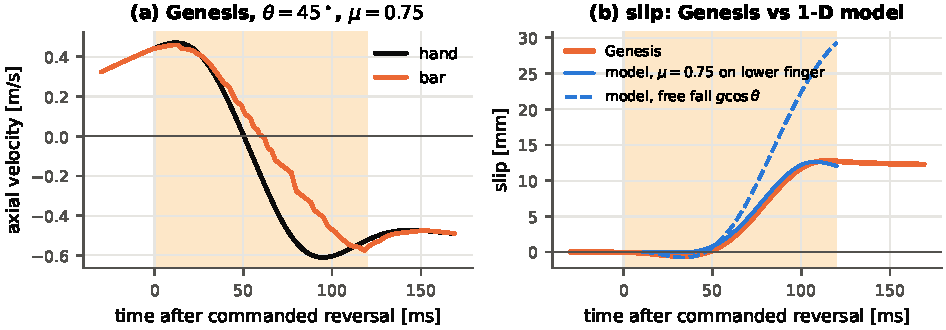
\includegraphics[width=\linewidth]{figs/physics.pdf}
\caption{One scripted throw in Genesis at $45^\circ$, $\mu=0.75$, logged at \SI{1}{kHz}. (a) Hand and bar
velocities along the axis; shading marks the forced-open window. (b) Slip against the 1-D model \eqref{eq:rel}
driven by the measured hand velocity.}
\label{fig:physics}
\end{figure}

\subsection{What limits the slip per throw}
Figure~\ref{fig:sweep} scripts the throw in Genesis across peak speed and open window. At $v=\SI{0.45}{m/s}$
the best slip is \SIrange{11}{13}{mm} at every tilt, reached with a \SIrange{100}{120}{ms} window. The policy's
window is \SI{120}{ms} forced and up to \SI{160}{ms} loose, so it sits at or past that optimum. The
companion report (\emph{Pulse Duration versus Arm Velocity}) derives the matched condition
$v^*=\tfrac12\gp T_p$. For a \SIrange{120}{160}{ms} window it asks for \SIrange{0.6}{0.8}{m/s}. With the cap
lifted to \SI{0.65}{m/s}, Genesis gives \SIrange{24}{25}{mm} per throw at $45^\circ$ for windows of 120 to
\SI{160}{ms}. That is more than the largest target (\SI{22.5}{mm}), so any target is reachable in one throw,
with the peak speed as the knob that scales it down.

\begin{figure}[!htb]
\centering
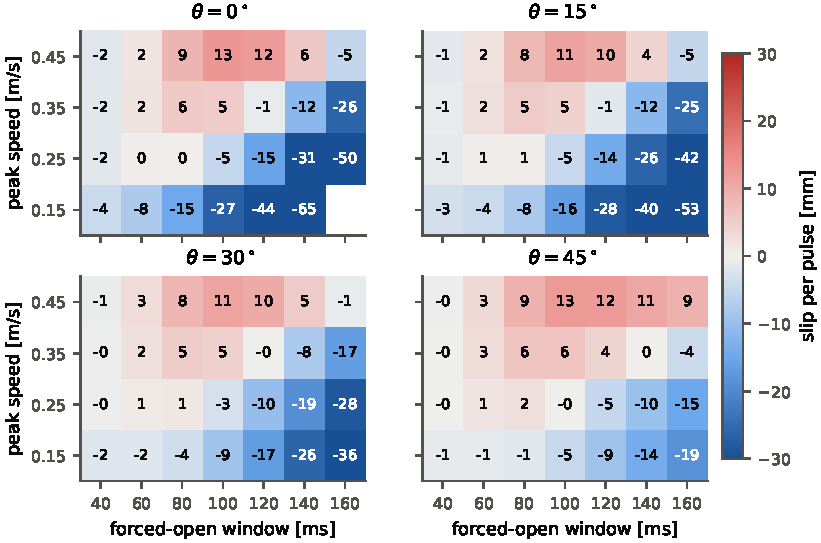
\includegraphics[width=\linewidth]{figs/sweep.pdf}
\caption{Genesis, scripted throws: slip per pulse [mm] against peak speed and forced-open window, trigger at the
commanded reversal. Blank cell: that environment reset before re-grip.}
\label{fig:sweep}
\end{figure}

%==========================================================================
\section{Transfer to the real FR3}
%==========================================================================
The learned behaviour reaches the robot as an open-loop replay of policy trajectories. Four pieces in
\code{franka\_controllers} make the real cell reproduce the simulated start state and motion:
\begin{itemize}
\item \textbf{Homing} (\code{home\_fr3v2.py --tilt-deg}, \code{tilted\_homing.py}). Joints 1--4 take the
simulation values. Joints 5--7 are solved on the real URDF and gripper mounting so that the grasp direction
matches. A hand-calibrated pose is used at $30^\circ$.
\item \textbf{The simulation's reset and the datum of a CSV} (\code{sim\_home\_tilted.py}). The simulator
integrates from $v(0)=0$ with the trapezoid rule, so the pose to home to is
$z_0=\code{target\_z}[0]-\tfrac12\code{target\_z\_vel}[0]\,T$. For the exported $45^\circ$ episode this equals
$Z_0$ to within $2\times10^{-7}$\,m. The script also checks the travel envelope against joint limits with the
controller's own damped least squares.
\item \textbf{Axis-following control} (\code{motion\_mode: fixed\_axis}, \code{\textasciitilde/axis\_vel\_cmd}). This
is the same structure as the simulator's controller: the scalar speed is rotated onto a fixed line, with
transverse position feedback and the orientation held at activation.
\item \textbf{Replay} (\code{replay\_traj\_csv.py}) streams \code{target\_z\_vel} at \SI{50}{Hz} and fires one Robotiq
pulse per open window.
\end{itemize}
\textbf{What does not transfer automatically.}
\begin{itemize}
\item The gripper is different: a Robotiq 2F on the robot, the Franka hand model in simulation. Its latency and
effective open time are not yet measured.
\item The real reference chain adds one command period of interpolation lag. The reversal at \SI{112.5}{ms} of
the test profile falls between publish ticks.
\item The contact friction of the real bar on the real pads is unknown, and Eq.~\eqref{eq:rel} shows the slip
depends on it strongly.
\end{itemize}
The companion report quantifies all three and gives the measurements that close them. Closed-loop deployment
of the policy would also need the in-hand offset $r_z$ on the robot, for example from the motion-capture setup in
\code{hrii\_optitrack}.

%==========================================================================
\section{Recommendations}
%==========================================================================
\begin{enumerate}
\item \textbf{Raise \code{Z\_VEL\_MAX} to about \SI{0.65}{m/s}, or shorten the open window to about
\SI{80}{ms}.} Either choice matches the throw to the pulse (Section~\ref{sec:physics}). The first gives about
\SI{24}{mm} per throw in Genesis, enough to finish in one pulse and worth roughly $1.9\times$ the discounted
return of a two-pulse success (5343 vs 2858). Check the height budget first: a faster throw travels further.
\item \textbf{Consider rescaling the regrasp bonus.} The quartic bonus reaches \SI{9.1e3}{} at the largest
target, close to the success reward. A policy that becomes able to make large single throws will be driven
mostly by the bonus.
\item \textbf{Fix the stale test and comment.} Five tests in \code{test\_env\_franka\_parallel\_tilted.py} target a
\code{progress\_reward} term that the environment does not define (it uses \code{proximity\_reward}). They fail
now: 12 of 17 pass. The proximity comment still quotes the $M=20$ values.
\item \textbf{Observe the tilt when training across angles.} $\theta$ is fixed per run and absent from the
observation. A single multi-tilt policy would need it, or would need to infer it through the GRU.
\end{enumerate}

\appendix
%==========================================================================
\section{Constants}
%==========================================================================
\begin{center}\small
\begin{tabular}{llll}
\toprule
policy / sim period & \SI{20}{ms} / \SI{1}{ms} & episode & 450 steps (\SI{9}{s})\\
$v_{\max}$, $a_{\max}$ & \SI{0.45}{m/s}, \SI{15}{m/s^2} & filter $\omega_n,\zeta$ & \SI{75}{rad/s}, 0.33\\
$K_{\text{ax}}, K_{\text{tr}}, K_r, \lambda$ & 8, 80, 40, $10^{-4}$ & joint $k_p$ & 4500/3500/2000\\
fingers closed / open & 0.251 / \SI{13.0}{mm} & finger $k_p$, $k_v$ & $\mathcal U[100,500]$, 25\\
pulse $D$, $L$ & 2, 7 steps & lockout, start block & 60, 50 steps\\
release / firm force & 0.15 / \SI{0.75}{N} & regrasp limit & fail on 7th; bonus on first 4\\
$R_s$, $c_t$, $c_a$, $R_{\text{to}}$, $F$ & $10^4$, 0.5, 1.25, 250, 912.5 & proximity $M,R,k$ & 30, \SI{50}{mm}, 5\\
smoothness weights & 25, 25; refund 6, free 9 & speed, blockade & 2.25; settle 0.3, prep \SI{0.2}{s}\\
friction $\mu$ & $\mathcal U[0.6,0.9]$ & target $r_z^*$ & $\mathcal U[12.5,22.5]$\,mm\\
\bottomrule
\end{tabular}
\end{center}

%==========================================================================
\section{Reproduction}
%==========================================================================
\begin{verbatim}
# train (genesis container)
python3 examples/rigid/train_franka_ppo_gru.py --env env_franka_parallel_tilted \
        --tilt-deg 45 -e tilt45-gru-speed --normalization --randomize -B 1024
# unit tests (no scene is built)
cd examples/rigid && python3 -m unittest test_env_franka_parallel_tilted
# Genesis throw experiments, then figures and this PDF
python3 reports/tools/pulse_slip_sweep.py --tilts 0 15 30 45 \
        --out reports/data/pulse_slip.npz
python3 reports/tools/pulse_hires.py --tilts 0 40 45 \
        --out reports/data/pulse_hires.npz
python3 reports/rl_tilted/make_figs.py
cd reports/rl_tilted && latexmk -pdf rl_tilted_regrasp_report.tex
\end{verbatim}
Learning curves are read from the runs' TensorBoard files into \code{reports/data/tb\_curves.npz}. All quoted
numbers are written to \code{reports/rl\_tilted/numbers.json}.

\end{document}
